%770
\newpage
\subsection{例題4-2 ミニサッカーゲームのボールや色を変える}

\begin{description}
    \item \textgt{\bf 考え方}
\end{description}

ミニサッカーゲーム(kick.hsp)のプログラムを改造してゲームの内容を変えてみましょう。

ゲームの中に出てくるサッカーボールもmes命令によって表示されています。


\begin{figure}[H]
    \begin{center}
      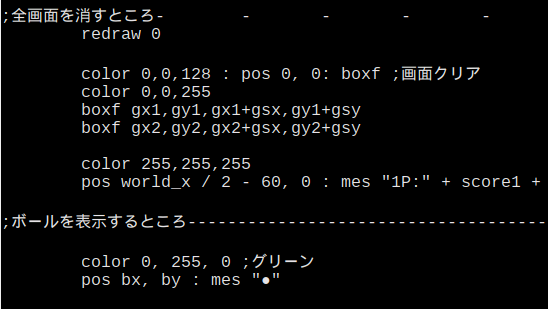
\includegraphics[keepaspectratio,width=14.499cm,height=8.123cm]{text04-img/s_kicksrc2.png}
      \caption{ミニサッカーゲームのプログラム}
    \end{center}
    \label{fig:prog_menu}
\end{figure}


このボールも変えることができます。

プログラムの中から、ボールを出している部分を探して変更しましょう。



color命令は、色を決める命令だということを覚えていますか?

第2回で覚えたcolor命令の使い方を思い出しながら、ボールの色を変えてみましょう。


\begin{figure}[H]
    \begin{center}
      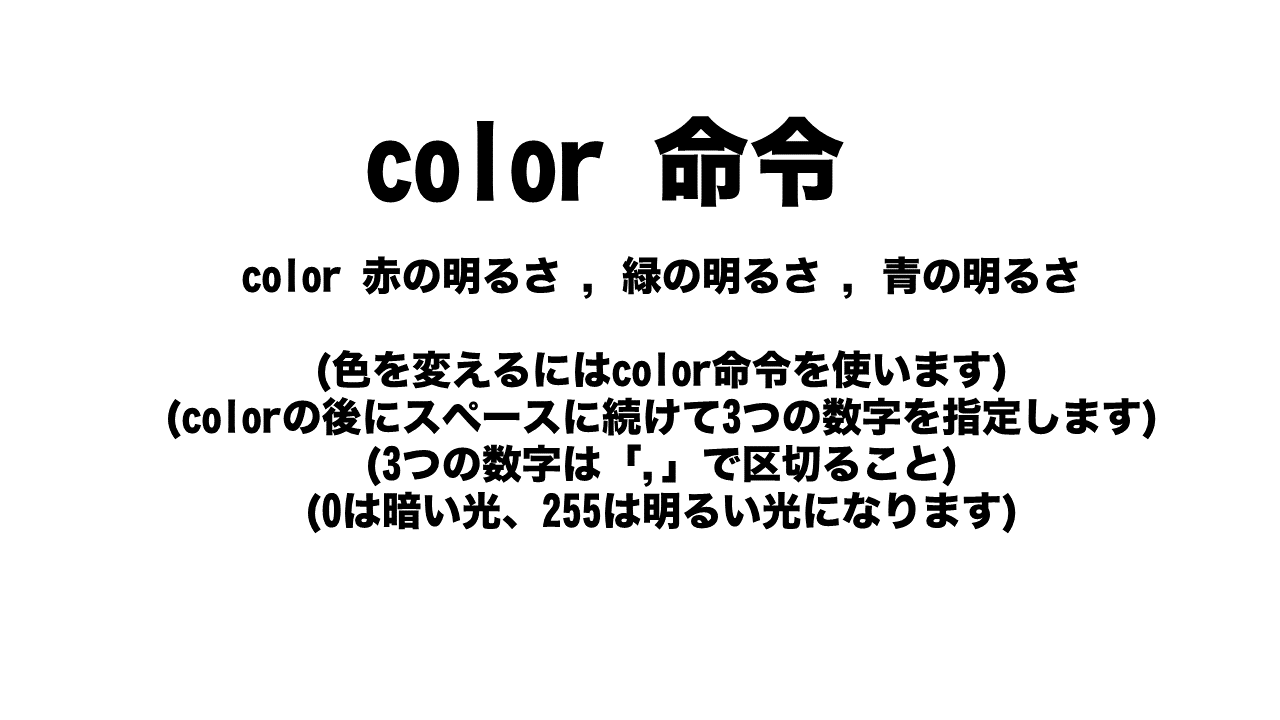
\includegraphics[keepaspectratio,width=12.409cm,height=7.62cm]{text04-img/s_kicksrc3.png}
    \end{center}
    \label{fig:prog_menu}
\end{figure}


このゲームでは画像を一切使っていません。

背景のゴール、人、ボールも含めてすべてプログラムの中で決めています。

boxf命令は、好きな大きさの\ruby{四角形}{し|かく|けい}を画面に出すことのできる命令です。

この命令とcolorを組み合わせて背景となる色やゴールを出しています。



\ruby{実際}{じっ|さい}に色を書き\ruby{換}{か}えて、オリジナルのサッカーゲームを作ってみましょう。

タイトルの文字や、得点を表示する文字も変えることができます。




\begin{description}
    \item \textgt{\bf 例題4-2 答え}
\end{description}


[F5]キーを押して改造した部分がきちんと表示されるかどうか確認しましょう。

\ \ \ \ プログラムを改造することで、見た目が変わってあなただけのゲームに変わります。

改造ができたらTAや周りの友達にも見せてあげましょう。